In this section we will test other clustering algorithm on the data, visualizing how they perform in comparison with the spectral clustering performed above.

\subsection{Plain \textit{Kmeans} Algorithm}
Performing the plain \textit{K-means} algorithm on our data yields poor results since the algorithm is based on euclidean distance. This is the reason it fails to recognize shapes other than balls.

\begin{figure}[H]
    \centering
    \subfloat[1][\textit{K-means} algorithm performed on \texttt{circle}]{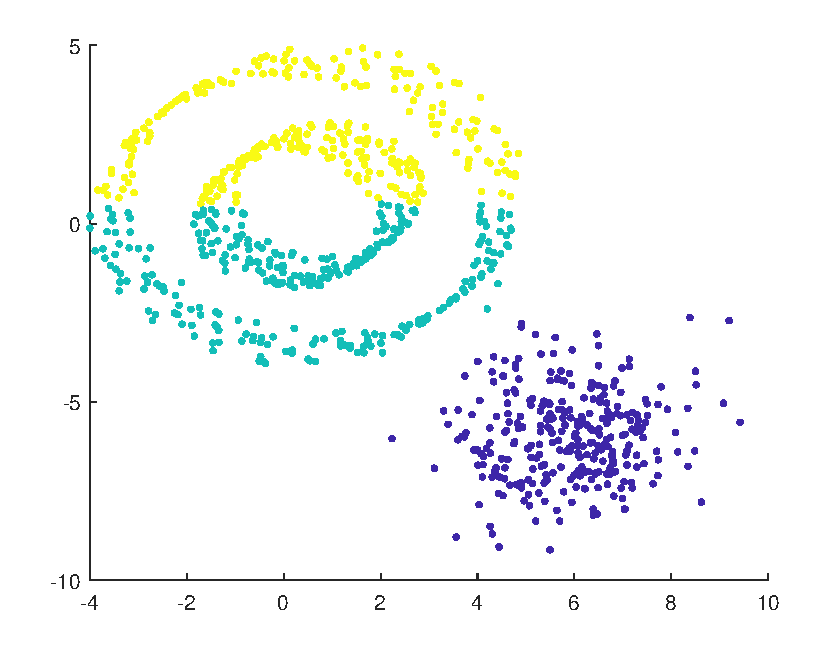
\includegraphics[scale = 0.45]{pictures/circle_Kmeans_nospectral.pdf}}
    \qquad
    \qquad
    \subfloat[2][\textit{K-means} algorithm performed on \texttt{spiral}]{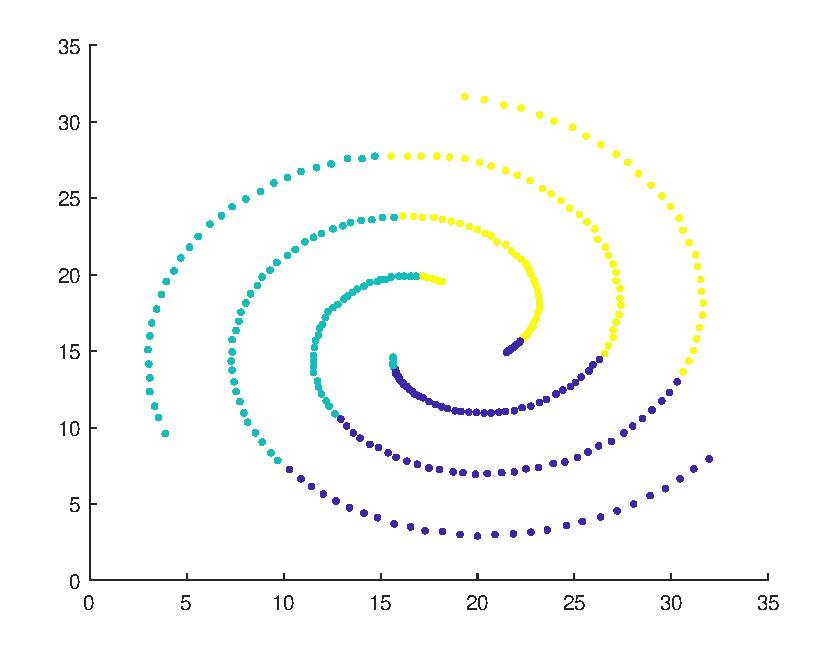
\includegraphics[scale = 0.45]{pictures/spiral_Kmeans_nospectral.pdf}}
    \caption{\textit{K-means} algorithm performed onto the datasets}
    \label{kmeans_nospectral}
  \end{figure}

  As it is clearly visible in figure \ref{kmeans_nospectral}, the \textit{K-means} algorithm performed on spatial data is only able to recognize the cloud of points in the \texttt{circle} data since is euclidean-ball shaped. It clearly fails to recognize any other shape and this results in a very poor clustering with regard to shaped data.

  \subsection{DBSCAN algorithm}
  The DBSCAN algorithm is an "explorative" approach to clustering. Without going into details, at its core the DBSCAN algorithm populate each cluster by searching the neighborhood of each point in the cluster hence performs much better at recognizing shapes than the plain \textit{K-means} algorithm.

  \begin{figure}[H]
    \centering
    \subfloat[1][DBSCAN algorithm performed on \texttt{circle}]{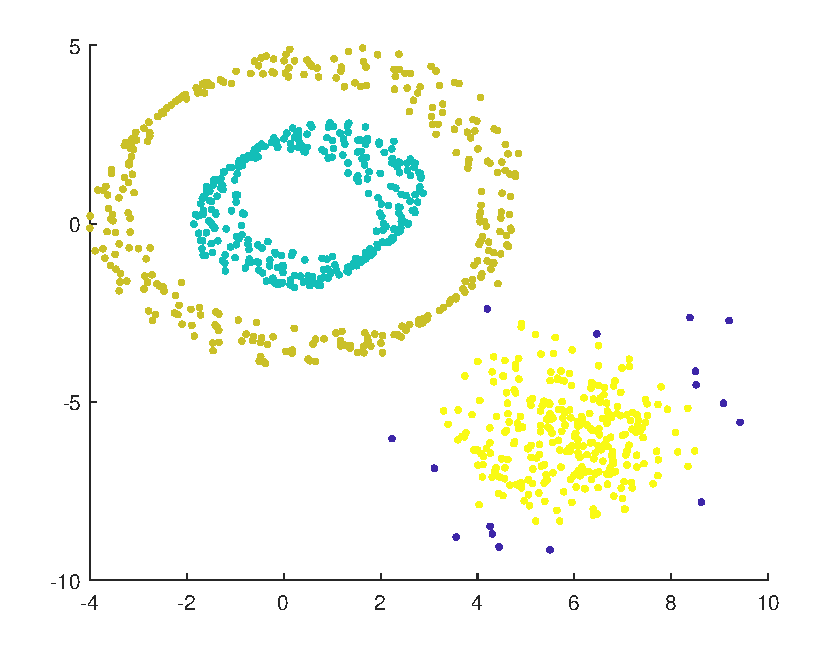
\includegraphics[scale = 0.45]{pictures/circle_dbscan_nospectral.pdf}}
    \qquad
    \qquad
    \subfloat[2][DBSCAN algorithm performed on \texttt{spiral}]{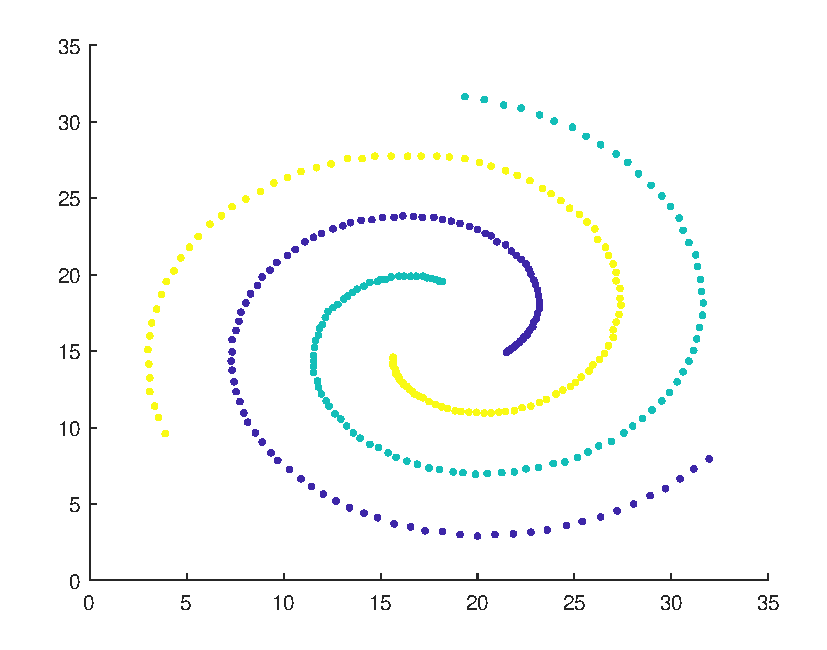
\includegraphics[scale = 0.45]{pictures/spiral_dbscan_nospectral.pdf}}
    \caption{DBSCAN algorithm performed onto the datasets}
    \label{dbscan_nospectral}
  \end{figure}

  \noindent The results of the clustering are shown in Figure \ref{dbscan_nospectral}. Those are obtained using the \texttt{dbscan} function in MATLAB performing some minor tuning of the parameters. In particular the clustering for the \texttt{circle} data was obtained using the default metric of the algorithm which is the euclidean distance while for the \texttt{spiral} data the Mahalanobis distance was used.
  \\
  \\
As it is visible in Figure \ref{dbscan_nospectral} the DBSCAN algorithm is perfectly capable of recognizing shapes and correctly classifies all points of the two datasets with the only exception of some points in the \texttt{circle} dataset. 
